\hypertarget{SurrogateSplits_8h}{
\section{Surrogate\-Splits.h File Reference}
\label{SurrogateSplits_8h}\index{SurrogateSplits.h@{SurrogateSplits.h}}
}


This graph shows which files directly or indirectly include this file:\begin{figure}[H]
\begin{center}
\leavevmode
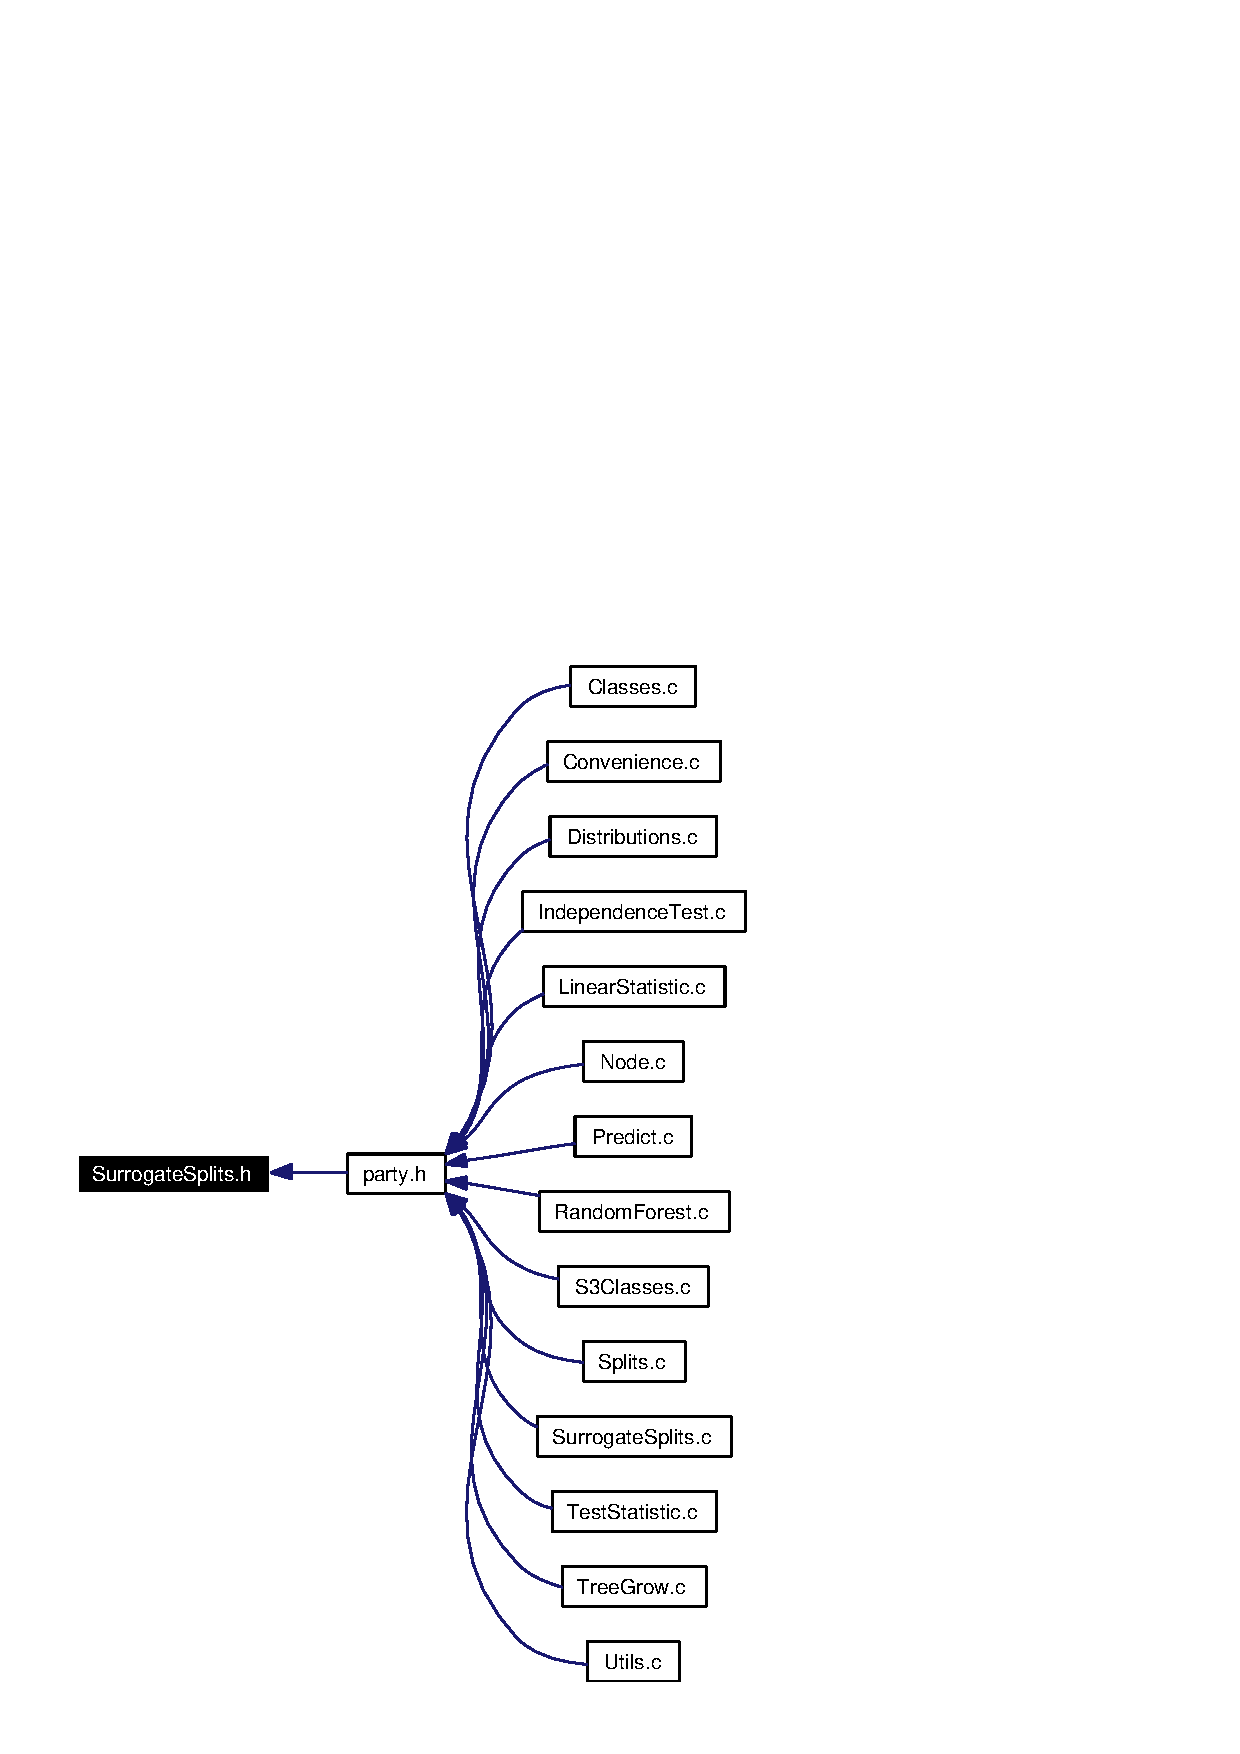
\includegraphics[width=179pt]{SurrogateSplits_8h__dep__incl}
\end{center}
\end{figure}
\subsection*{Functions}
\begin{CompactItemize}
\item 
void \hyperlink{SurrogateSplits_8h_fd8931db67339ca2bb679d8d38135275}{C\_\-surrogates} (SEXP node, SEXP learnsample, SEXP weights, SEXP controls, SEXP fitmem)
\item 
void \hyperlink{SurrogateSplits_8h_6f9f8c3b4147854cacc43d67a055d911}{C\_\-splitsurrogate} (SEXP node, SEXP learnsample)
\end{CompactItemize}


\subsection{Function Documentation}
\hypertarget{SurrogateSplits_8h_6f9f8c3b4147854cacc43d67a055d911}{
\index{SurrogateSplits.h@{Surrogate\-Splits.h}!C_splitsurrogate@{C\_\-splitsurrogate}}
\index{C_splitsurrogate@{C\_\-splitsurrogate}!SurrogateSplits.h@{Surrogate\-Splits.h}}
\subsubsection[C\_\-splitsurrogate]{\setlength{\rightskip}{0pt plus 5cm}void C\_\-splitsurrogate (SEXP {\em node}, SEXP {\em learnsample})}}
\label{SurrogateSplits_8h_6f9f8c3b4147854cacc43d67a055d911}


Split with missing values \par
 \begin{Desc}
\item[Parameters:]
\begin{description}
\item[{\em node}]the current node with primary and surrogate splits specified \item[{\em learnsample}]learning sample \end{description}
\end{Desc}


Definition at line 169 of file Surrogate\-Splits.c.

References get\_\-missings(), get\_\-nobs(), get\_\-variable(), has\_\-missings(), PL2\_\-inputs\-Sym, S3get\_\-leftnode(), S3get\_\-nodeweights(), S3get\_\-primarysplit(), S3get\_\-rightnode(), S3get\_\-splitpoint(), S3get\_\-surrogatesplits(), S3get\_\-toleft(), and S3get\_\-variable\-ID().

Referenced by C\_\-Tree\-Grow().

Here is the call graph for this function:\begin{figure}[H]
\begin{center}
\leavevmode
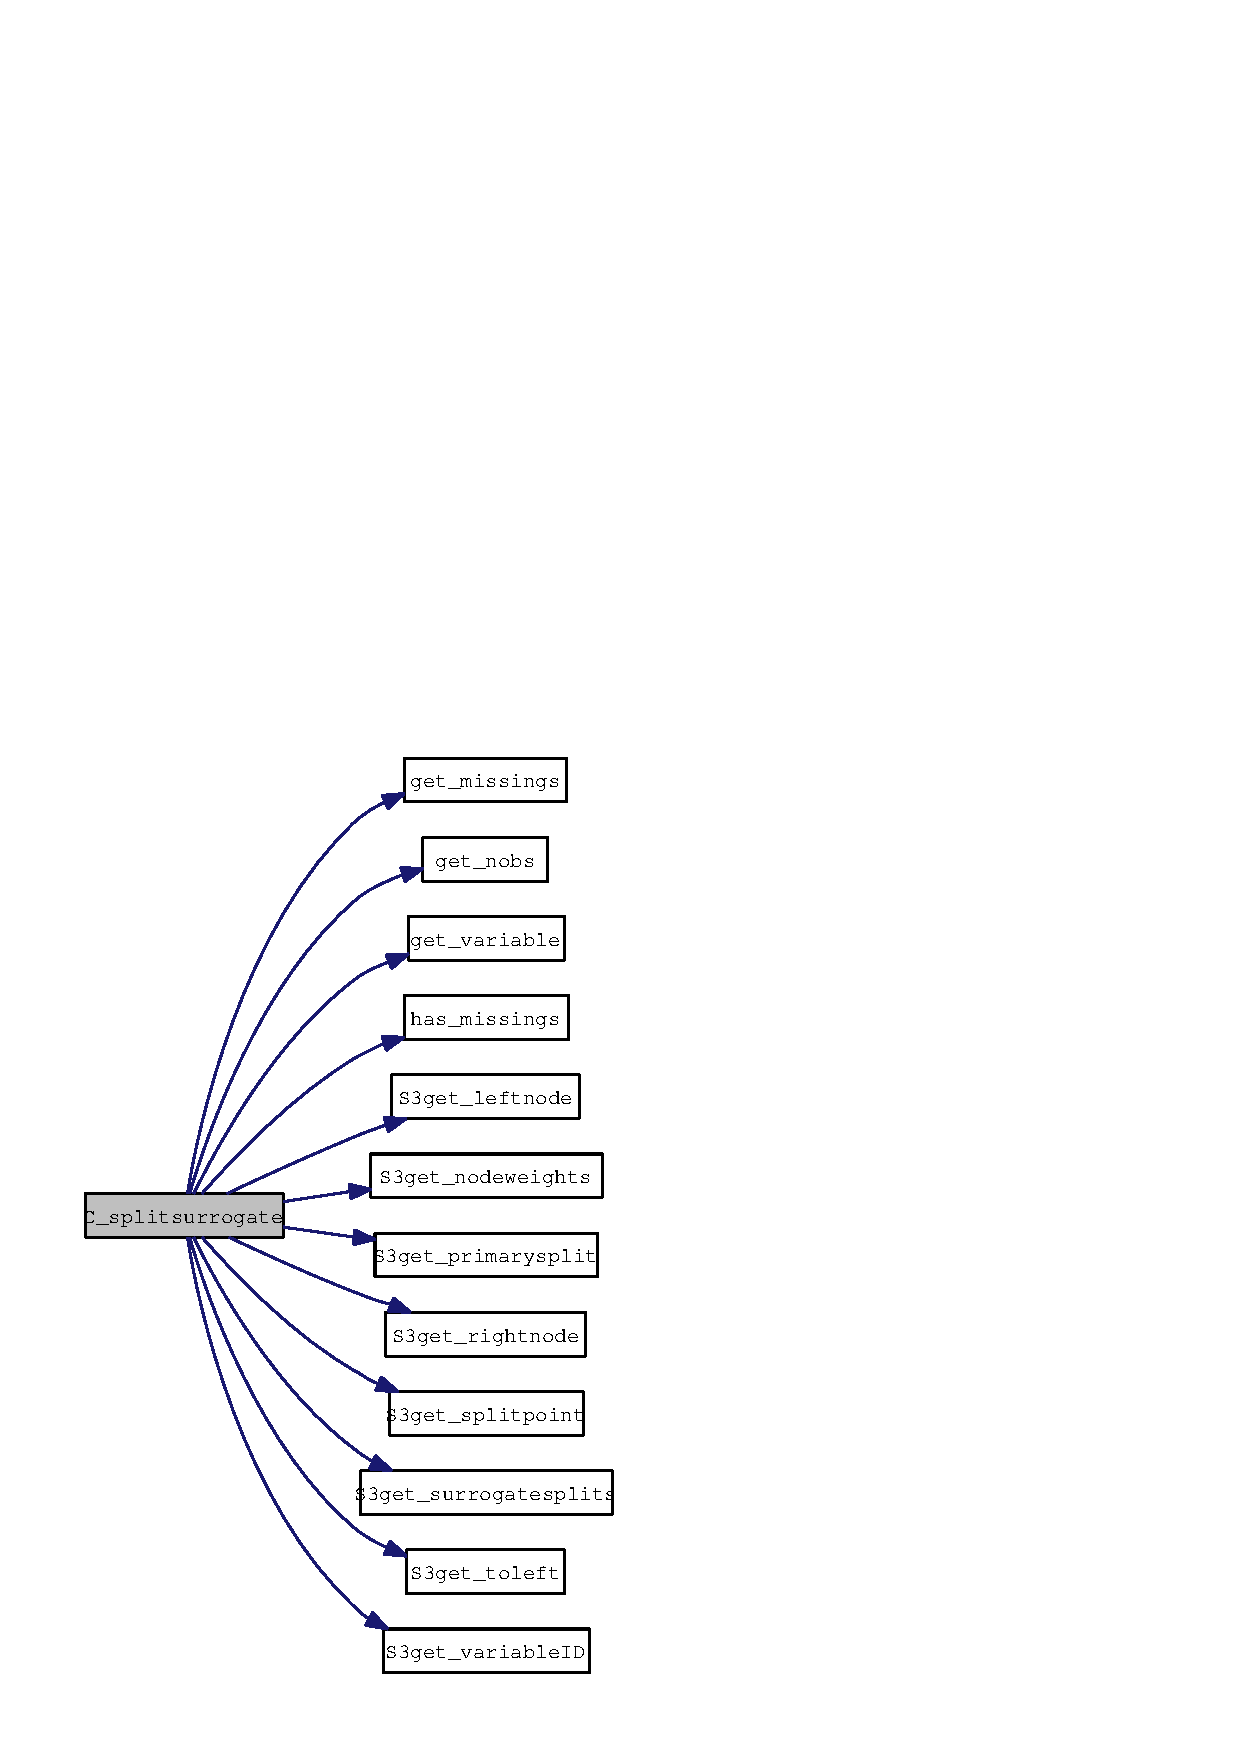
\includegraphics[width=195pt]{SurrogateSplits_8h_6f9f8c3b4147854cacc43d67a055d911_cgraph}
\end{center}
\end{figure}
\hypertarget{SurrogateSplits_8h_fd8931db67339ca2bb679d8d38135275}{
\index{SurrogateSplits.h@{Surrogate\-Splits.h}!C_surrogates@{C\_\-surrogates}}
\index{C_surrogates@{C\_\-surrogates}!SurrogateSplits.h@{Surrogate\-Splits.h}}
\subsubsection[C\_\-surrogates]{\setlength{\rightskip}{0pt plus 5cm}void C\_\-surrogates (SEXP {\em node}, SEXP {\em learnsample}, SEXP {\em weights}, SEXP {\em controls}, SEXP {\em fitmem})}}
\label{SurrogateSplits_8h_fd8931db67339ca2bb679d8d38135275}


Search for surrogate splits for bypassing the primary split \par
 \begin{Desc}
\item[Parameters:]
\begin{description}
\item[{\em node}]the current node with primary split specified \item[{\em learnsample}]learning sample \item[{\em weights}]the weights associated with the current node \item[{\em controls}]an object of class `Tree\-Control' \item[{\em fitmem}]an object of class `Tree\-Fit\-Memory' \end{description}
\end{Desc}
\begin{Desc}
\item[\hyperlink{todo__todo000003}{Todo}]enable nominal surrogate split variables as well \end{Desc}


Definition at line 21 of file Surrogate\-Splits.c.

References get\_\-maxsurrogate(), get\_\-missings(), get\_\-ninputs(), get\_\-nobs(), get\_\-splitctrl(), has\_\-missings(), PL2\_\-inputs\-Sym, S3get\_\-nodeweights(), S3get\_\-primarysplit(), S3get\_\-surrogatesplits(), and S3get\_\-variable\-ID().

Referenced by C\_\-Tree\-Grow(), and R\_\-surrogates().

Here is the call graph for this function:\begin{figure}[H]
\begin{center}
\leavevmode
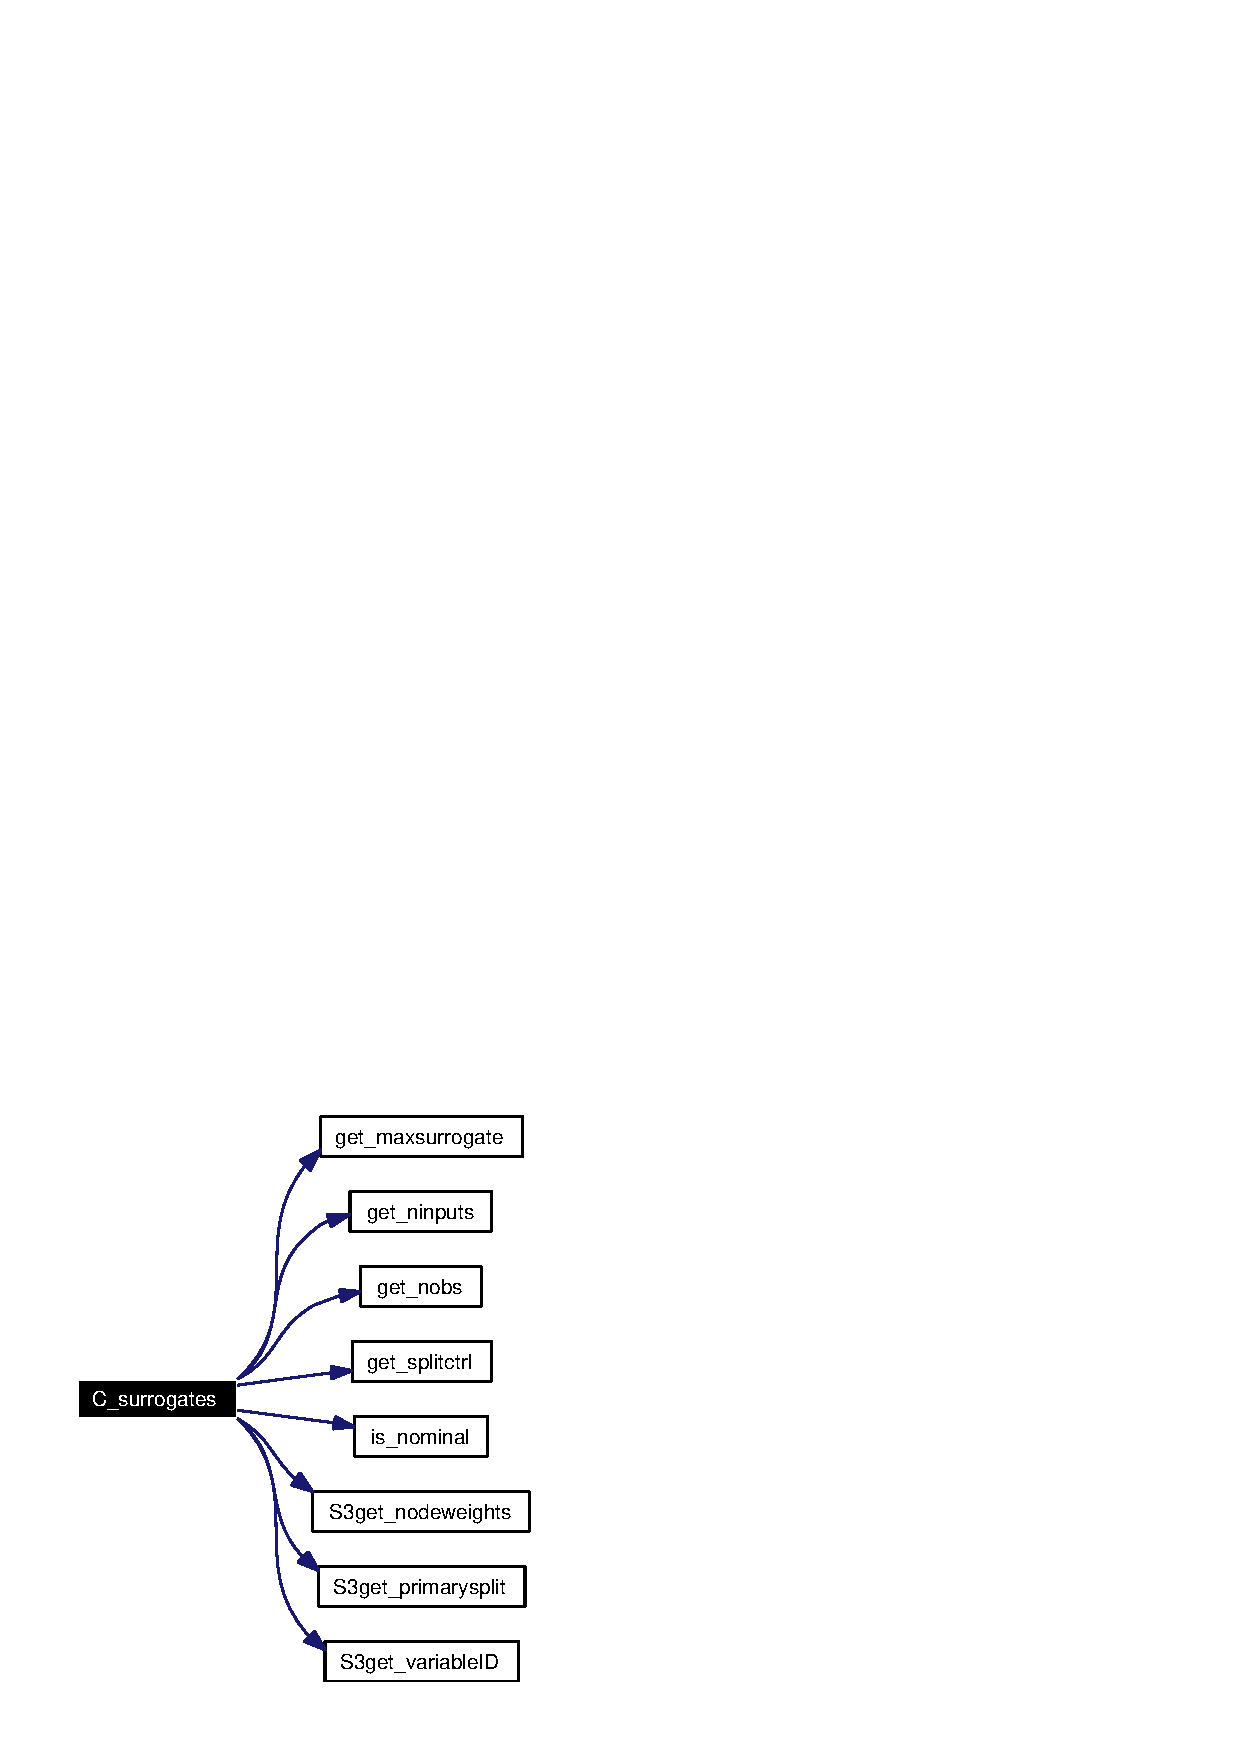
\includegraphics[width=189pt]{SurrogateSplits_8h_fd8931db67339ca2bb679d8d38135275_cgraph}
\end{center}
\end{figure}
